% % say that lammps and matlab were used in Introduction

\documentclass[BTech]{iitmdiss}
\usepackage{textcomp}
\usepackage{times}
%\usepackage{breqn}
\usepackage{tabularx}
\usepackage{url}
\usepackage{rotating}
\usepackage{adjustbox}
\usepackage{mathtools}
%\usepackage{geometry}
\usepackage{pbox}
\usepackage{multirow}
%\usepackage[paper=a4paper,left=1.5in,right=1in,top=1in,bottom=0.667in,nohead]{geometry}
\usepackage{float}
\usepackage{t1enc}
\usepackage{wrapfig}
\usepackage{graphicx}
\usepackage{epstopdf}
\usepackage{lipsum}
\newcommand{\startsquarepar}{%
    \par\begingroup \parfillskip 0pt \relax}
\newcommand{\stopsquarepar}{%
    \par\endgroup}
\usepackage[driverfallback=dvipdfm]{hyperref} % hyperlinks for references.
\usepackage{amsmath} % easier math formulae, align, subequations \ldots
\ProvideTextCommand{\DJ}{OT1}{\raisebox{0.25ex}{-}\kern-0.4em D}
\usepackage{paracol}
\usepackage{subfig}
\usepackage{siunitx}


\usepackage{pgfplots}
\pgfplotsset{compat=1.15}
\usepackage{mathrsfs}
\usepackage{color}
\usepackage{csquotes}
\usetikzlibrary{arrows}
\newcommand{\degre}{\ensuremath{^\circ}}

\definecolor{cqcqcq}{rgb}{0.7529411764705882,0.7529411764705882,0.7529411764705882}
\definecolor{ffqqqq}{rgb}{1,0,0}



\begin{document}

%%%%%%%%%%%%%%%%%%%%%%%%%%%%%%%%%%%%%%%%%%%%%%%%%%%%%%%%%%%%%%%%%%%%%%
% Title page
    \newcommand{\titleText}{Remote Center of Motion Constrained Planning for a 7DOF Robotic Arm}
    \newcommand{\authorText}{Suraj Rathi}
    \title{\titleText}

    \author{\authorText}

    \date{25 May 2023}
    \department{Mechanical Engineering}

%\nocite{*}
%\RequirePackage[ %compat2,a4paper,left=1.5in,right=1in,top=1in,bottom=0.667in,                nohead]{geometry}[2002/07/08]
    \newgeometry{left=1in,right=1.5in,top=1in,bottom=0.667in}
    \maketitle

%%%%%%%%%%%%%%%%%%%%%%%%%%%%%%%%%%%%%%%%%%%%%%%%%%%%%%%%%%%%%%%%%%%%%%
% Declaration
    \declaration

    \vspace*{0.5in}

    \noindent I certify that the ideas, designs, experimental work, results, analyses and conclusions set out in this
    dissertation are entirely my own effort, except where otherwise indicated and acknowledged.
    I further certify that the work is original and has not been previously submitted for assessment in
    any other course or institution, except where specifically stated.

    \vspace*{0.5in}


    \begin{paracol}{2}
        \vspace*{1.0in}
        \begin{singlespacing}
            \hspace*{-0.25in}
            \parbox{2.5in}{
                \noindent Place: Chennai\\
                Date: 25$^{\textnormal{th}}$ May 2023
            }
        \end{singlespacing}

        \switchcolumn
        \begin{singlespacing}
            \includegraphics[height=1.0in]{/home/suraj/Documents/abhiyaan/ros/src/btp/report/img/signature}


            \hspace*{-0.25in}
            \parbox{2.5in}{
                \noindent Name: Suraj Surendra Rathi \\
                \noindent Roll No. ME19B177
            }


        \end{singlespacing}

    \end{paracol}

%%%%%%%%%%%%%%%%%%%%%%%%%%%%%%%%%%%%%%%%%%%%%%%%%%%%%%%%%%%%%%%%%%%%%%
% Certificate
    \certificate

    \vspace*{0.5in}

    \noindent This is to certify that the thesis titled {\bf \titleText}, submitted by {\bf \authorText},
    to the Indian Institute of Technology, Madras, for
    the award of the degree of {\bf B.Tech}, is a bona fide
    record of the research work done by him under my supervision. The
    contents of this thesis, in full or in parts, have not been submitted
    to any other Institute or University for the award of any degree or
    diploma.

    \vspace*{1.5in}

    \begin{paracol}{2}
        \begin{singlespacing}
            \hspace*{-0.25in}
            \parbox{2.5in}{
                \noindent {\bf Dr.\ Nirav Patel} \\
                \noindent Research Guide \\
                \noindent \textit{Assistant Professor} \\
                \noindent Dept. of Engineering Design\\
                \noindent IIT-Madras, 600 036
            }
            \hspace*{1.56in}

            \vspace*{0.3in}
            \noindent Place: Chennai\\
            Date: 25$^{\textnormal{th}}$ May 2023

        \end{singlespacing}

        \switchcolumn
        \begin{singlespacing}
            \hspace*{-0.25in}
            \parbox{2.5in}{
                \noindent {\bf Dr.\ Sathyan Subbiah} \\
                \noindent Research Guide \\
                \noindent \textit{Professor} \\
                \noindent Dept. of Mechanical Engineering\\
                \noindent IIT-Madras, 600 036
            }
            \hspace*{1.56in}

            \vspace*{0.3in}
            \noindent Place: Chennai\\
            Date: 25$^{\textnormal{th}}$ May 2023

        \end{singlespacing}

    \end{paracol}

%%%%%%%%%%%%%%%%%%%%%%%%%%%%%%%%%%%%%%%%%%%%%%%%%%%%%%%%%%%%%%%%%%%%%%
% Acknowledgements
    \newgeometry{left=1.5in,right=1in,top=1in,bottom=0.667in}
    \acknowledgements

    I would like to thank my guides, Dr.\ Nirav Patel, Dept of Engineering Design, and Dr.\ Sathyan Subbiah, Dept. of Mechanical Engineering for their guidance and support throughout this project.
    Nirav Sir has been supporting me on every aspect of my work from day one, providing valuable experience from his long career.
    Whenever we are at a fork in the road, sir has always been able to provide valuable insights on which direction to proceed.
    I am forever grateful for the knowledge I gained while working under him.


%%%%%%%%%%%%%%%%%%%%%%%%%%%%%%%%%%%%%%%%%%%%%%%%%%%%%%%%%%%%%%%%%%%%%%
% Abstract

    \abstract

    \noindent KEYWORDS: \hspace*{0.5em} \parbox[t]{4.4in}{Path Planning; Inverse Kinematics; KUKA LBR iiwa R800}

    \vspace*{24pt}
    \noindent
    In this project we attempt to build a realtime path planner satisfying a remote center of motion constraint.
    After ensuring the method will converge to a solution, the optimization objective is to minimize the total joint motion and to enforce motion limits on each joint.
    We set up a simulation using Open Robotics’ Gazebo to conduct our experiments in conjunction with the ROS platform.
    We worked to identify the challenges faced by planning in task space using Inverse-Kinematics.
    Sampling based methods were then used to improve the performance.
    Our work demonstrates the effectiveness of task space Inverse-Kinematics based methods.



    \pagebreak

    \disclaimer
    The Department of Mechanical Engineering, IIT Madras and the staff of IIT Madras, do not accept any responsibility for the truth, accuracy or completeness of material contained within or associated with this dissertation.

    Persons using all or any part of this material do so at their own risk, and not at the risk of the Department of Mechanical Engineering, IIT Madras and the staff of IIT Madras,

    This document, the associated hardware, software, drawings, and other material set out in the associated appendices should not be used for any other purpose: if they are so used, it is entirely at the risk of the user

    \pagebreak


%%%%%%%%%%%%%%%%%%%%%%%%%%%%%%%%%%%%%%%%%%%%%%%%%%%%%%%%%%%%%%%%%
% Table of contents etc.

    \begin{singlespace}
        \tableofcontents
        \thispagestyle{empty}

        \listoftables
        \addcontentsline{toc}{chapter}{LIST OF TABLES}
        \listoffigures
        \addcontentsline{toc}{chapter}{LIST OF FIGURES}
    \end{singlespace}


%%%%%%%%%%%%%%%%%%%%%%%%%%%%%%%%%%%%%%%%%%%%%%%%%%%%%%%%%%%%%%%%%%%%%%
% Abbreviations
    \newpage
    \begin{tabbing}

    \end{tabbing}
    \abbreviations

    \noindent
    \begin{tabbing}
        xxxxxxxxxxxxxx \= xxxxxxxxxxxxxxxxxxxxxxxxxxxxxxxxxxxxxxxxxxxxxxxx \kill
        \textbf{RCM} \> Remote Center of Motion\\
        \textbf{DOF} \> Degrees of Freedom\\

    \end{tabbing}

    \pagebreak

% %%%%%%%%%%%%%%%%%%%%%%%%%%%%%%%%%%%%%%%%%%%%%%%%%%%%%%%%%%%%%%%%%%%%%%
% % Notation
%
%     \chapter*{\centerline{NOTATIONS}}
%     \addcontentsline{toc}{chapter}{NOTATIONS}
%
%     \begin{singlespace}
%         \begin{tabbing}
%             xxxxxxxxxxx \= xxxxxxxxxxxxxxxxxxxxxxxxxxxxxxxxxxxxxxxxxxxxxxxx \kill
%             $F$ \>  Force (N)\\
%             $\delta$ \> Displacement (m)\\
%
%         \end{tabbing}
%     \end{singlespace}
%
%     \pagebreak
%     \clearpage

% The main text will follow from this point so set the page numbering
% to arabic from here on.
    \pagenumbering{arabic}


%%%%%%%%%%%%%%%%%%%%%%%%%%%%%%%%%%%%%%%%%%%%%%%%%%
% Introduction.


    \chapter{INTRODUCTION}\label{ch:intro}


    \section{Motivation}\label{sec:motiv}
    Laparoscopic surgery, commonly know as `keyhole' surgery, is a procedure where a surgeon accesses the inside of
    the abdomen and pelvis without having to make a large incision.
    We are attempting to use a LBR iiwa 7~[\cite{AG}] arm produced by KUKA, which is a 7DOF robotic arm, to perform such a surgery.

    In this surgery, a small incision is made on the skin, and the surgical instruments are manipulated through that incision.
    We have model this as a cylindrical, and later circular, shape.
    The endeffector must always enter through the upper circular face and exit through the lower circular face.
    It must always pass through some volume of the cylinder and cannot intersect with the curved surface.
    An illustration can be seen in~\ref{fig:RCM}.
    This is quite similar to the `Remote Center of Motion' (RCM) constraint and henceforth, when we use the term RCM we will be referring to the aforementioned constraint.

    \begin{figure}
        \centering
        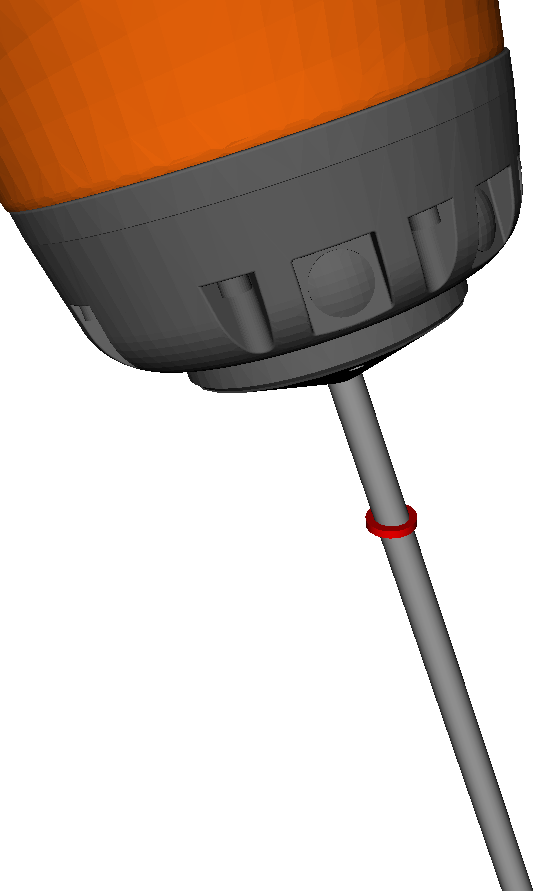
\includegraphics[height= 0.5\textwidth]{./img/rcm-constraint}
        \caption{A depiction of the Laproscopic surgery constraint as implemented in our work. The orange and gray objects are part of the robotic arm and the red cylinder represents the volume through which the end-effector must always pass.}
        \label{fig:RCM}
    \end{figure}

    We wished to implement a real-time path planner that can satisfy the RCM constraint.


    \section{Survey of Existing Methods}

    \subsection{Path Planners}
    Our survey of existing planning methods was primarily done by surveying the available algorithms in ROS MoveIT [\cite{Coleman_Sucan_Chitta_Correll_2014}].
    This library provides a unified frontend to various motion planners and integrates wil the FCL collision checker, and with simulation and visualization software through the ROS framework.
    We must note that these planners are optimized for a general purpose use case.
    Our robot is very simple, and when it is inside the RCM, we observed that the links do not collide with each-other we do not require all the complexities and features of these full scale planners.

    A second technique can be used, wherein if we can generate a path in task space (i.e. in the coordinates of the tip of the end-effector),
    we can use Inverse Kinematics (IK) to generate the required joint angles in configuration space. This approach generally has the following problems.
    \begin{enumerate}
        \item Solving the IK problem may be slow
        \item There may be no IK solution for a given pose
        \item The IK solution will not be unique
        \item There may be large jumps in IK solutions between two consecutive points in the path.
    \end{enumerate}

    The Kinematics and Dynamics Library (KDL)~[\cite{kdl-url}] is default solver used by MoveIT for solving forward and inverse kinematics problems.
    We can also use the IKFast algorithm to generate analytical solutions for a given robot configuration.

    \subsection{7DOF Robot Control}

    Another challenge with working with this robot is its the over-actuated nature.
    To control the six DOF of the end-effector pose, we need to specify the joint angle of seven actuators.
    This leaves us with one extra DOF.
    In literature, we have seen others use that DOF to implement better obstacle avoidance~[\cite{Doliwa_2020}] and lock a single joint to get closed form kinematics~[\cite{Asthana}]


    \section{Objectives}

    \begin{enumerate}
        \item Build a simulated environment using the KUKA LBR iiwa 7 with the RCM constraint in Gazebo and integrate it with the ROS MoveIT framework.
        \item Identify challenges with implementing the RCM constraint using task-space planning and Inverse Kinematics.
        \item Implement and test the effectiveness of a sampling based technique to minimize the joint motion along the path.
    \end{enumerate}


    \section{Risk Assessment}\label{sec:risk}

    The algorithm has been developed and tested on a simulated environment built in Gazebo.
    We have not taken any extra measures to ensure the reliable operation on real hardware.
    The above algorithm has also only been tested on the given workspace configuration.
    Results may vary with different robot models, workspace positioning, and RCM placement.
    The modeled RCM may not accurately resemble the characteristics in real life.


    \section{Resource Requirements}
    The following resources were used to complete this work:
    \begin{itemize}
        \item ROS Catkin Environment
        \item Gazebo Simulator
        \item (If Possible for testing) KUKA LBR iiwa R800
    \end{itemize}


    \chapter{METHODOLGY}\label{ch:method}


    \section{Simulation Building}

    We built our simulation using the Gazebo~[\cite{gazebo-url}] simulator.
    It is a widely-used open-source robotics simulator that provides a realistic 3D environment for developing and testing robot algorithms.

    We used~\cite{hennersperger2017towards} as the basis of the simulated environment and added a needle shaped end-effector and a ellipsoidal model of an abdomen.
    The initial simulation environment is seen in \ref{fig:initial_simulation_models}.
    The `abdomen' model enforces the RCM constraint.

    \begin{figure}
        \centering
        \subfloat[\centering End Effector]{{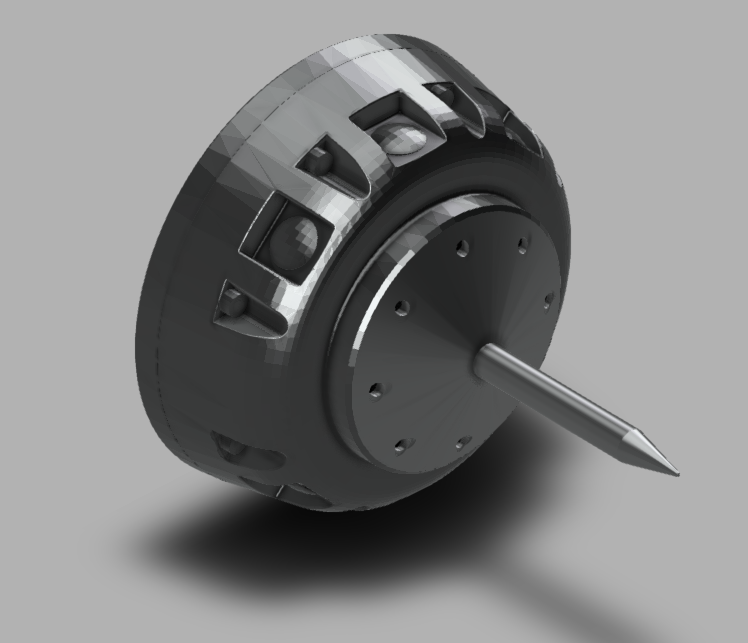
\includegraphics[height=0.25 \linewidth]{./img/initial_endeffector}}}%=
        \qquad
        \subfloat[\centering Abdomen]{{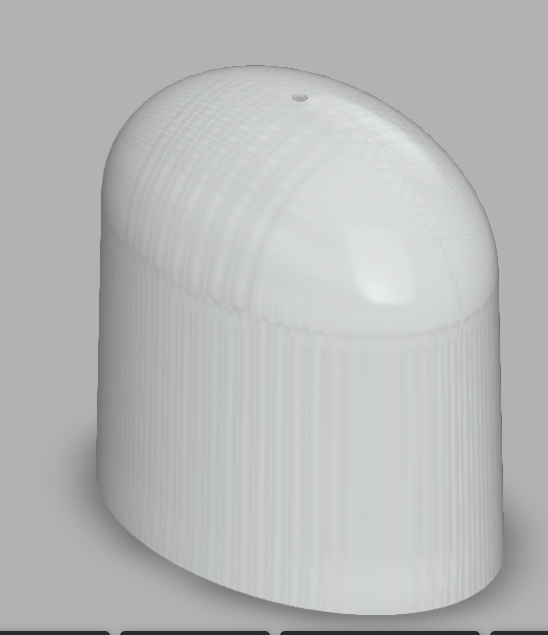
\includegraphics[height=0.25 \textwidth]{./img/initial_abdomen}}}%
        \qquad
        \subfloat[\centering Visualization]{{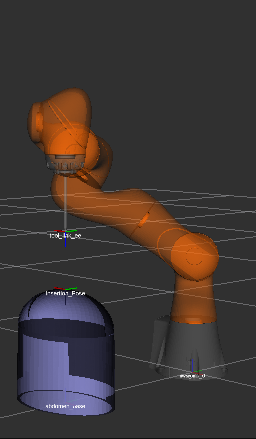
\includegraphics[height=0.25 \textwidth]{./img/initial_sim_env_viz}}}
        \caption{The initial models for use in simulation}
        \label{fig:initial_simulation_models}
    \end{figure}

    The models were slowly changed as the project progressed to better model the problem of Laparoscopic surgery.
    The dimensions of the end effector were changed to a length of \SI{350}{\milli\meter} and base radius of \SI{2}{\milli\meter} (\ref{fig:longer_ee}).

    \begin{figure}
        \centering
        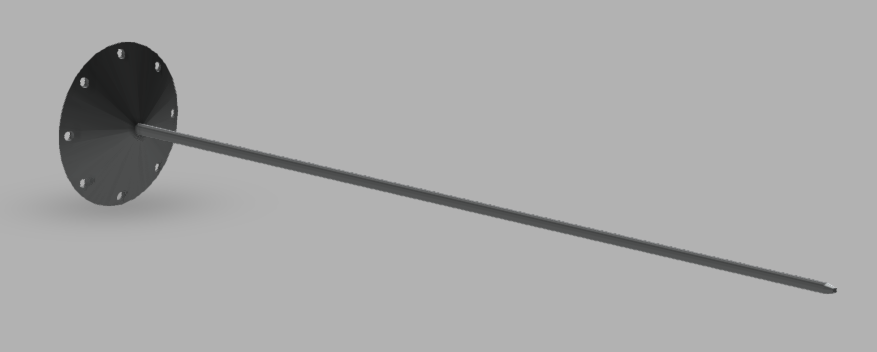
\includegraphics[width=0.75 \linewidth]{./img/longer_end_effector}
        \caption{The longer end effector.}
        \label{fig:longer_ee}
    \end{figure}

    Another major change in the simulation was to change the cylindrical RCM \ref{fig:rcm_cylinder} to a circular RCM \ref{fig:rcm_circle}.
    The circular model can be represented as the cylindrical model where the height of the cylinder is 0.

    \begin{figure}
        \centering
        \input{./img/rcm_cylinder.txt}
        \caption{The original cylindrical RCM model. The red region represents the RCM and the gray region represents the end effector.}
        \label{fig:rcm_cylinder}
    \end{figure}

    \begin{figure}
        \centering
        \input{./img/rcm_circle.txt}
        \caption{The new circular RCM model. The red region represents the RCM and the gray region represents the end effector.}
        \label{fig:rcm_circle}
    \end{figure}

    With this setup, we were able to run the full ROS MoveIT planning stack with generic algorithms.
    However, using the mesh as a constraint for the RCM is extremely slow, and this naive approach would not run in real-time.


    \section{Inverse Kinematics}

    As is used by ROS MoveIT, we leveraged the KDL library for solving the forward and inverse kinematic models.
    Do note that we are using a patched version of the pyKDL library, see Appendix~\ref{ch:code}.

    The KDL library uses an implementation of `Differential Inverse Kinematics'.
    In this method the SVD decomposition of the Jacobian is used to calculate the configuration space velocity for a given task space velocity.
    With this, the Newton-Raphson method is used to find an IK solution (configuration-space state) given a prior state.

    We found that in practice, this method provided the following:
    \begin{enumerate}
        \item Real-time solutions to the IK problem.
        \item A deterministic and unique IK solution.
        \item No large jumps in solutions because of the gradient based nature of the technique
    \end{enumerate}

    The final guarantee that still needs to be shown, is that we must be able to find an IK solution at all points in the workspace.
    Firstly, based on the RCM constrataint model, we can take the workspace as the combination of a cone with its apex at the RCM
    and axis along the vertical and a spherical cap with its center as the cone's apex.
    With the RCM constraint, we have a limited workspace area (figure \ref{fig:workspaces}), so we can discretize the workspace and check whether a
    solution can be found.

    \begin{figure}
        \centering
        \subfloat[\centering First Test]{{\includegraphics[height=0.25 \linewidth]{./img/initial_workspace}}}%=
        \qquad
        \subfloat[\centering Long Needle Test]{{\includegraphics[height=0.25 \textwidth]{./img/long_needle_ws}}}%
        \qquad
        \subfloat[\centering Final Workspace]{{\includegraphics[height=0.25 \textwidth]{./img/final_ws}}}
        \caption{The workspace defined for each test. The cone is the reachable volume, and the cylinder represents the region we considered in our experiments.}
        \label{fig:workspaces}
    \end{figure}
    We used an implementation of floodfill to iterate through all states in the workspace, starting from an initial state
    and use the IK solver to calculate a solution and store the total change in joint angle, position error, and orientation error.
    The IK solver is seeded from the IK solution of the previous state.
    The implementation with a FIFO queue ensures that for a given state, the IK solution is seeded by that of a state which is closer to the starting point.

    If the joint values at each point were of small enough magnitude, then we get a weak guarantee of it possible to find an IK solution at each point.
    The guarantee is weak as we are only checking from an initial point outwards, not from any point A to another adjacent point.


    \section{RCM Implementation}

    \subsection{Simple Implementation}\label{subsec:simple-rcm-impl}

    As input to the IK routine, we need to provide a 6DOF pose.
    This consists of the end effector's cartesian position and orientation.
    The cartesian position is provided to us as the input to the algorithm (target point).
    This leaves us with 3DOF from the orientation to implement the RCM constraint.
    As seen in figure \ref{fig:target_orientation}, we've taken a ray from the center of the upper face of the RCM to the target point.
    We then find the smallest rotation transforming a coordinate axis such that the x axis will lie along that vector.

    \begin{figure}
        \centering
        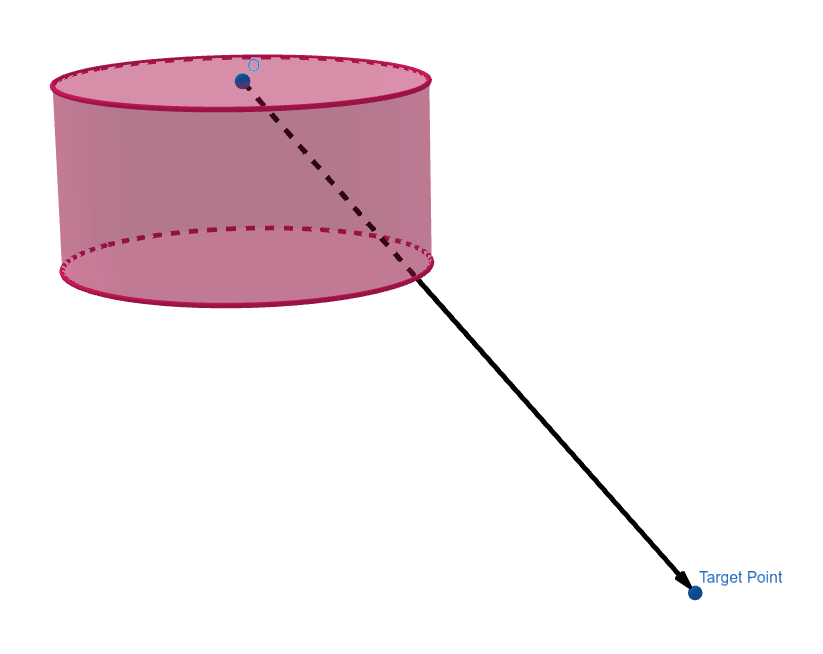
\includegraphics[width=0.5 \linewidth]{./img/target_orientation}
        \caption{The black vector shows the required orientation of the end effector. The pink cylinder represents the RCM constraint.}
        \label{fig:target_orientation}
    \end{figure}


    In ROS, rotations between two coordinate frames are represented as quaternions.
    We need to find the quaternion that represents the minimum rotation between the base frame and the target frame.
    See figure \ref{fig:coordinate_frames} for reference.
    Let $\vec{O}$ represent the center of the upper face of the cylinder and $\vec{t}$ represent the target position.
    From equation \ref{eqn:final_q}, we can get the final expression for the orientation as a quaternion.
    In the implementation we have had add support for special cases where this expression can approach $\infty$.

    \begin{align}
        \vec{d} &= \vec{t} - \vec{O} \\
        \vec{l} &= \frac{(0, 0, -1) \times \vec{d}}{|\vec{d}|} \\
        \theta &= \arccos{\left(\frac{(0, 0, -1) \cdot \vec{d}}{|\vec{d}|}\right)} \\
        \mathbf{q} &= \cos{\frac{\theta}{2}} + \left(l_x \mathbf{i} + l_y \mathbf{j} + l_z \mathbf{k} + \right) \sin{\frac{\theta}{2}} \label{eqn:final_q}
    \end{align}


    \begin{figure}
        \centering
        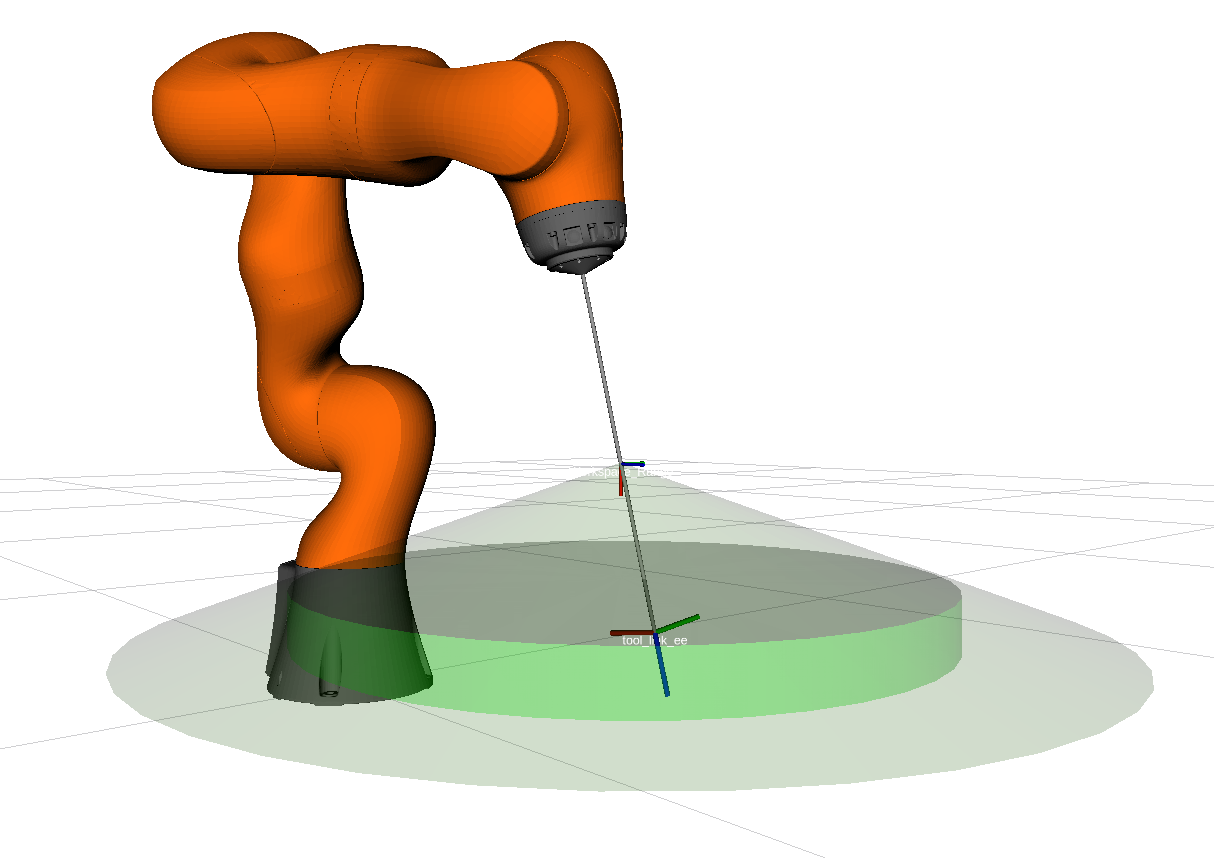
\includegraphics[width=0.5 \linewidth]{./img/coordinate_frames}
        \caption{The set of red, green, and blue line segments represent the x, y, and z axes of a coordinate frame.
        The upper frame is the frame of reference (base frame) for the target frame.}
        \label{fig:coordinate_frames}
    \end{figure}

    \subsection{Sampling Based Implementation}\label{sec:sampling_rcm}

    % TODO: Add an image showing different samples

    In section~\ref{subsec:simple-rcm-impl} we have taken an arbitrary point in the RCM through which the center of our
    end-effector must pass through.
    However, we know that the end effector can pass through any point in the upper face,
    as long as the end-effector will not intersect with the curved surface of the cylinder.
    We can then choose the point to minimize an optimization criterion.

    As the IK solver is a non-analytical technique, we cannot find an analytical solution for this technique.
    Instead, we can attempt to find the best point by random sampling. The process can be seen in figure \ref{fig:sampling_flowchart}.

    \begin{figure}
        \centering

        \input{./img/sampling_flowchart.txt}

        \caption{Flowchart depicting the Sampling based RCM implementation.}
        \label{fig:sampling_flowchart}
    \end{figure}

    A mathematical representation of the RCM constraints was developed for the cylindrical and circular case.
    Let the center of the upper face of the RCM be denoted by $\vec{O}$, the point we have chosen on the upper face be $\vec{P}$,
    the radius of the RCM $R$, the radius of the end-effector $r$, and the thickness of the RCM be $t$.
    The equation \ref{eqn:cylinder_cons} lays out the required condition for a cylindrical constraint.
    In the implementation, we have taken care to handle the cases where we are dividing by the norm of a very small vector.

    \begin{align}
        \vec{O'} &= \vec{O} + (0, 0, -t) \\
        \vec{Q'} &= \vec{Q} - (\vec{P} - \vec{Q}) * \frac{t}{P_z - Q_z} \\
        d_{upper} &= (R - |\vec{Q} - \vec{O}|) * \frac{|(\vec{P} - \vec{Q}) \times (\vec{O} - \vec{Q})|}{|\vec{P} - \vec{Q}| |\vec{O} - \vec{Q}|} \\
        d_{lower} &= (R - |\vec{Q'} - \vec{O'}|) * \frac{|(\vec{P} - \vec{Q'}) \times (\vec{O'} - \vec{Q'})|}{|\vec{P} - \vec{Q'}| |\vec{O'} - \vec{Q'}|} \\
        \text{is\_valid} &= (d_{upper} > r) \land (d_{lower} > r)\label{eqn:cylinder_cons}
    \end{align}

    When we later shifted to a circular constraint, we used just $d_{upper}$.
    The calls to the underlying vector mathematics library (numpy) were manually inlined and unrolled to increase speed.


    \chapter{RESULTS}\label{ch:results}


    \section{Feasibility of Inverse Kinematics Based Methods}\label{sec:flood_fill}

    The primary test conducted over the course of this project was to check whether IK would succeed over all points in a given workspace.
    We tested this for a variety of configurations of different needle lengths, workspace locations, RCM configurations, and number of samples.
    The most important results are shown below.

    In the following tests, the mentioned algorithm was used to compute the joint angles for each point in the workspace.
    The IK algorithm was seeded by the closest point in the direction of the starting point.
    The computation was started from the bottom center of the workspace, and a breadth-first search like algorithm (floodfill)
    was used to iteratively cover each point in the workspace.
    The total difference in the joint angles from the seed point, position error, and orientation error were stored.




    \emph{First Test:} In this test, we used a short needle and a small (restrictive) RCM\@.
    The test showed that the algorithm was able to find a solution at every point in the workspace.
    Figure~\ref{fig:initial_test} shows the distribution of the joint motion angles as a box and whisker plot.
    We wish to minimize this value to ensure a smoother path.
    The experiment had a maximum joint motion of \SI{2.58}{\degre}, maximum position error on the order of \SI{e-15}{\meter},
    and a maximum orientation error of \SI{e-6}{\degre}.
    This shows that for this case, the IK algorithm is well-equipped to provide path planning solutions.

    \begin{figure}

        \centering
        \subfloat[\centering Workspace]{{ \includegraphics[width=0.35 \linewidth]{./img/initial_workspace}}}
        \qquad
        \subfloat[\centering Joint Angle Distribution]{{ \includegraphics[width=0.35 \linewidth]{./img/exp_1_boxplot}}}
        \centering
        \caption{The results from the `First Test'.}
        \label{fig:initial_test}z
    \end{figure}

    We tested the results with the following four configurations with different number of samples:
    \begin{enumerate}
        \item ``No Sampling''
        \item ``Sample, No Collision'': Sampling without RCM Collision Checking
        \item ``Sampling''
        \item ``Sample Center First'': Sampling with the center of the RCM as the first sample.
    \end{enumerate}
    We found that there was almost a negligible difference in techniques 2, 3, and 4.
    The resulting plots can be seen in figure \ref{fig:sampling_techniques}.
    There was a clear improvement in performance with number of samples (figure \ref{fig:initial_num_samples}),
    but the base case of no samples out performed each sampling based technique.

    \begin{figure}
        \centering
        \includegraphics[width=0.8 \linewidth]{./img/sampling_techniques}
        \caption{The performance of different sampling techniques for `First Test'.}
        \label{fig:sampling_techniques}
    \end{figure}

    \begin{figure}
        \centering
        \includegraphics[width=0.8 \linewidth]{./img/initial_num_samples}
        \caption{For `First Test', the performance with number of samples.}
        \label{fig:initial_num_samples}
    \end{figure}

    \emph{Long Needle Test:} The above experiment was then repeated with a longer end-effector to more accurately model the surgical procedure.
    The results (figure \ref{fig:long_needle_box}) were similar to the `First Test' but there was a large set of failures  (table \ref{tab:failure_rate}).
    We notice that the failure rate does seem to decrease with the number of samples, but is still unacceptably large.
    \begin{table}[h]
        \centering
        \begin{tabular}{|c|c|c|c|}
            \hline
            Number of Samples & None  & 10    & 100   \\ \hline
            Failure Rate (\%) & 19.20 & 19.15 & 19.02 \\ \hline
        \end{tabular}
        \caption{The failure rate with number of samples for the `Long Needle Test'.}
        \label{tab:failure_rate}
    \end{table}
    To better understand the failures, we plotted a 3d heatmap where the color of the cell indicates the total joint motion required to reach it from its neighbor.
    In figure \ref{fig:long_heatmap}. We can see that the failures are all seen on one side of the workspace on a smooth surface.
    We postulated that they could be caused due to incorrect workspace placement with respect to the robotic arm.

    \begin{figure}
        \centering
        \includegraphics[width=0.5 \linewidth]{/home/suraj/Documents/abhiyaan/ros/src/btp/report/img/long_needle_box}
        \caption{The results of the `Long Needle Test'.}
        \label{fig:long_needle_box}
    \end{figure}

    \begin{figure}
        \centering
        \includegraphics[width=0.5 \linewidth]{/home/suraj/Documents/abhiyaan/ros/src/btp/report/img/long_heatmap}
        \caption{The distribution of total joint motion across the workspace for the `Long Needle Test'.}
        \label{fig:long_heatmap}
    \end{figure}


    \emph{Shifted RCM Test:} We shifted the RCM to lie directly in front of the zero-angle position of the zeroth joint.
    This eliminated the problem we faced in the previous test.
    However, we found another region of very high joint in the form of a thin curved cylindrical region (Figure~\ref{fig:prefinal_heat}).

    \begin{figure}
        \centering
        \includegraphics[width=0.5 \linewidth]{/home/suraj/Documents/abhiyaan/ros/src/btp/report/img/prefinal_heat}
        \caption{Results for the `Shifted RCM Test'.}
        \label{fig:prefinal_heat}
    \end{figure}

    By visual inspection of the visualization, we found that this was caused by the robotic arm reaching a wrist joint singularity (Figure \ref{fig:wrist_singularity}).

    \begin{figure}
        \centering
        \includegraphics[width=0.4 \linewidth]{/home/suraj/Documents/abhiyaan/ros/src/btp/report/img/wrist_singularity}
        \caption{The robot in a wrist joint singularity state}
        \label{fig:wrist_singularity}
    \end{figure}

    \emph{Alternative Pose Test:} As the robot is an overactuated manipulator, there are an infinite combination of joint angles that
    can produce the same end-effector position.
    We had chosen an arbitrary state for the zero state in the workspace.
    We conducted this test (Figure \ref{fig:newpose}) with an alternate set of joint angles as the zero state and found
    that it brought down the joint motion by two to three times on average, and the problematic region had greatly reduced.

    \begin{figure}
        \centering
        \includegraphics[width=0.5 \linewidth]{/home/suraj/Documents/abhiyaan/ros/src/btp/report/img/newpose}
        \caption{The results with a different starting pose. Note that this figure has a different scale than the others.}
        \label{fig:newpose}
    \end{figure}


    \section{Sampling Based Implementation of the RCM Constraint}

    We assesed the performance of the sampling based algorithm discussed in section~\ref{sec:sampling_rcm} by
    comparing the path generated without sampling to that with sampling.
    We initially tested this on a straight line path (figure \ref{fig:straight_path}), and found no improvement with the algorithm.
    In fact, we found that the generated path was much less smooth.

    \begin{figure}
        \centering
        \includegraphics[width=0.8 \linewidth]{/home/suraj/Documents/abhiyaan/ros/src/btp/report/img/straight_path}
        \caption{The joint motion required for a straight line path with differnt number of samples.}
        \label{fig:straight_path}
    \end{figure}

    When we encountered the high joint angles due to the singularity in `Shifted RCM Test', we tested the planner with
    different number of samples along that path and along a slightly offset path (figure \ref{fig:ikpaths}).
    From the results in the figures~\ref{fig:forward_arc} and~\ref{fig:go_around},
    we can see that the sampling made the path worse when compared to no sampling,
    but within the sampling cases, a greater number of samples increased the path quality.

    \begin{figure}
        \centering
        \includegraphics[width=0.6 \linewidth]{/home/suraj/Documents/abhiyaan/ros/src/btp/report/img/ik_path_comparision}
        \caption{The paths along which the algorithm was tested. The center of the semicircle is the position of the singularity in this section.}
        \label{fig:ikpaths}
    \end{figure}

    \begin{figure}
        \centering
        \includegraphics[width=0.6 \linewidth]{/home/suraj/Documents/abhiyaan/ros/src/btp/report/img/forward_arc}
        \caption{Change in joint angle along the original path. Blue - no sampling, orange - 100 samples, green - 1000 samples.}
        \label{fig:forward_arc}
    \end{figure}

    \begin{figure}
        \centering
        \includegraphics[width=0.6 \linewidth]{/home/suraj/Documents/abhiyaan/ros/src/btp/report/img/go_around}
        \caption{Change in joint angle along the modified path.}
        \label{fig:go_around}
    \end{figure}


    \section{Runtime}

    By running a large number of iterations and finding the average time spent (Figure \ref{fig:runtime}), we found that our algorithm can run in
    realtime.
    We have also found that the position precision of the algorithm is well within the robot's repeatability.
    \begin{figure}
        \centering
        \includegraphics[width=0.6 \linewidth]{/home/suraj/Documents/abhiyaan/ros/src/btp/report/img/runtime}
        \caption{The speed at which the algorithm can be run on a Ryzen5 machine.}
        \label{fig:runtime}
    \end{figure}


    \chapter{CONCLUSION}\label{ch:conclusion}


    \section{Conclusion}

    Through the course of this work, we have found that Inverse Kinematics based methods are feasible for realtime path planning with the
    `Restricted Center of Motion' constraint and could possibly be used for Laparoscopic Surgery Robots.

    We found that the sampling technique we used to optimize the path did not bring about any improvements in the path.
    The greedy, single-step nature of the optimization is not useful in this use case.


    \section{Limitations and Future Work}

    The limitations of this work are already covered in section~\ref{sec:risk}.

    \noindent In the future, work must be carried out to look into the following.
    \begin{itemize}
        \item We should develop a more faithful model of the RCM that takes into account its elastic nature.
        \item An analytical model for points within the RCM that do not lead to a collision with the curved surface.
        (step two in figure~\ref{fig:sampling_flowchart}).
        \item Look into the effect of starting pose on the experiments done in section~\ref{sec:flood_fill}.
        \item Further understand and find techniques to mitigate the effect of singularities in the system.
        \item We can look into multistep optimization techniques to better optimize a path with the RCM constraint.
    \end{itemize}

%%%%%%%%%%%%%%%%%%%%%%%%%%%%%%%%%%%%%%%%%%%%%%%%%%%%%%%%%%%%
% Appendices.

    \appendix


    \chapter{Accessing and Running the Package} \label{ch:code}

    The source code for this work can be retried from Dr. Nirav Patel's lab at IIT Madras or at \texttt{https://github.com/surajRathi/KUKA\_RCM\_Control}
    To run this on Ubunutu 20.04, you need to install a patched version of the PyKDL library which can also be retrieved from Dr. Nirav's Lab.

    Run the following commands within a catkin workspace extended from an installation of ROS Noetic to correctly setup the package:


    \indent\texttt{git clone --recursive 'https:/github.com/surajRathi/KUKA\_RCM\_Control.git'}


    \indent\texttt{
        rosdep install --from-paths ./ --ignore-src catkin build iiwa\_needle\_moveit iiwa\_needle\_description iiwa\_tool\_description iiwa\_hw iiwa\_description iiwa\_gazebo iiwa\_moveit iiwa\_ros iiwa\_msgs iiwa\_control iiwa\_run
    }


    The files in the \texttt{iiwa\_run} package and the scripts in the same package are intended to be run.

    Please see the package for any further documentation.

    
%%%%%%%%%%%%%%%%%%%%%%%%%%%%%%%%%%%%%%%%%%%%%%%%%%%%%%%%%%%%
% Bibliography.

    \begin{singlespace}
        \bibliography{thesis_template}
        % \bibliographystyle{iitm}
    \end{singlespace}

\end{document}
